\documentclass[10pt]{beamer}

\mode<presentation>
{
 \usetheme{Boadilla}
\pagestyle{empty}

\setbeamerfont*{frametitle}{size=\normalsize,series=\bfseries}
\setbeamerfont*{block}{size=\normalsize,series=\bfseries}
%\setbeamertemplate{blocks}[rounded][shadow=true]
}

\definecolor{links}{HTML}{2A1B81}
\hypersetup{colorlinks,linkcolor=,urlcolor=links}


\usepackage{etex}
% \usepackage{helvet}
\usepackage{amsmath, amssymb}
\usepackage{color}
%\usepackage{asymptote}
\usepackage{mathrsfs}
\usepackage{dsfont}

\usepackage{pst-sigsys,pst-plot,pstricks-add}
%\usepackage{auto-pst-pdf}
\usepackage{pst-pdf}

\definecolor{links}{HTML}{2A1B81}
\hypersetup{colorlinks,linkcolor=,urlcolor=links}

\def\nn{\nonumber}

\definecolor{links}{HTML}{2A1B81}
\hypersetup{colorlinks,linkcolor=,urlcolor=links}

\newcommand{\fs}[2]{#2}

\title[]{Introduction to Systems.}
\author[\textcolor{blue}{Systems and Circuits}]{\textcolor{darkblue}{Pablo M. Olmos} (olmos@tsc.uc3m.es)\\ \textcolor{darkblue}{Emilio Parrado} (emipar@tsc.uc3m.es)}
\institute{\textcolor{white}{UC3M}}

\definecolor{darkblue}{rgb}{0.0, 0.0, 0.40}
\setbeamercolor{title}{fg=darkblue}
\setbeamercolor{frametitle}{fg=darkblue}
\definecolor{darkgreen}{rgb}{0.0, 0.4, 0.0}


\AtBeginSection[]
{
  \begin{frame}<beamer>{Index}
    \tableofcontents[currentsection,currentsubsection]
  \end{frame}
}

\begin{document}
\frame{
\titlepage
\thispagestyle{empty}
\begin{center}

\includegraphics[scale=0.05]{Figures/uc3m-logo.pdf}
\end{center}
}

\frame{

\frametitle{Systems}
\begin{itemize}
\item \textbf{System: Any process that results in the transformations of signals}.
\item Systems can model the behavior of a chemical process, a hydraulic system, an electric circuit, a communication channel, ...
\end{itemize}

}

\frame{
\frametitle{Microphone (transducer)}
\begin{figure}
\centering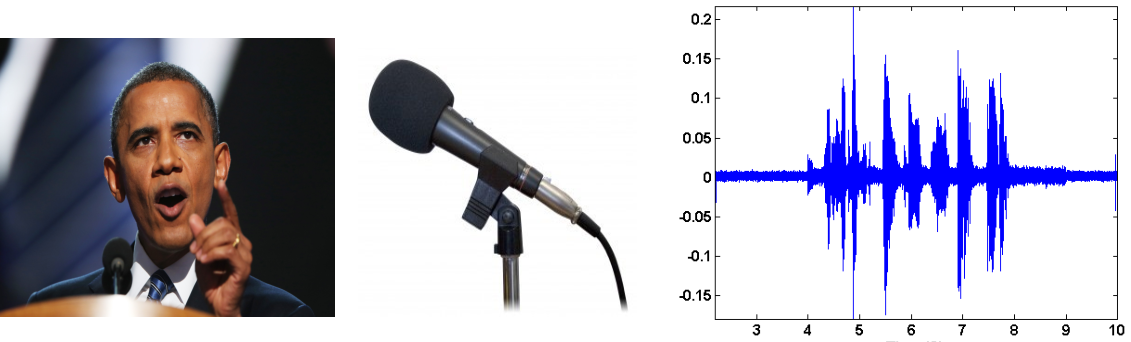
\includegraphics[scale=0.6]{Figures/Signal21.pdf}
\caption{Voice (pressure) signal $\Rightarrow$ Voltage signal}
\end{figure}
}

%\frame{
%\frametitle{Amplifer}
%\begin{figure}
%\centering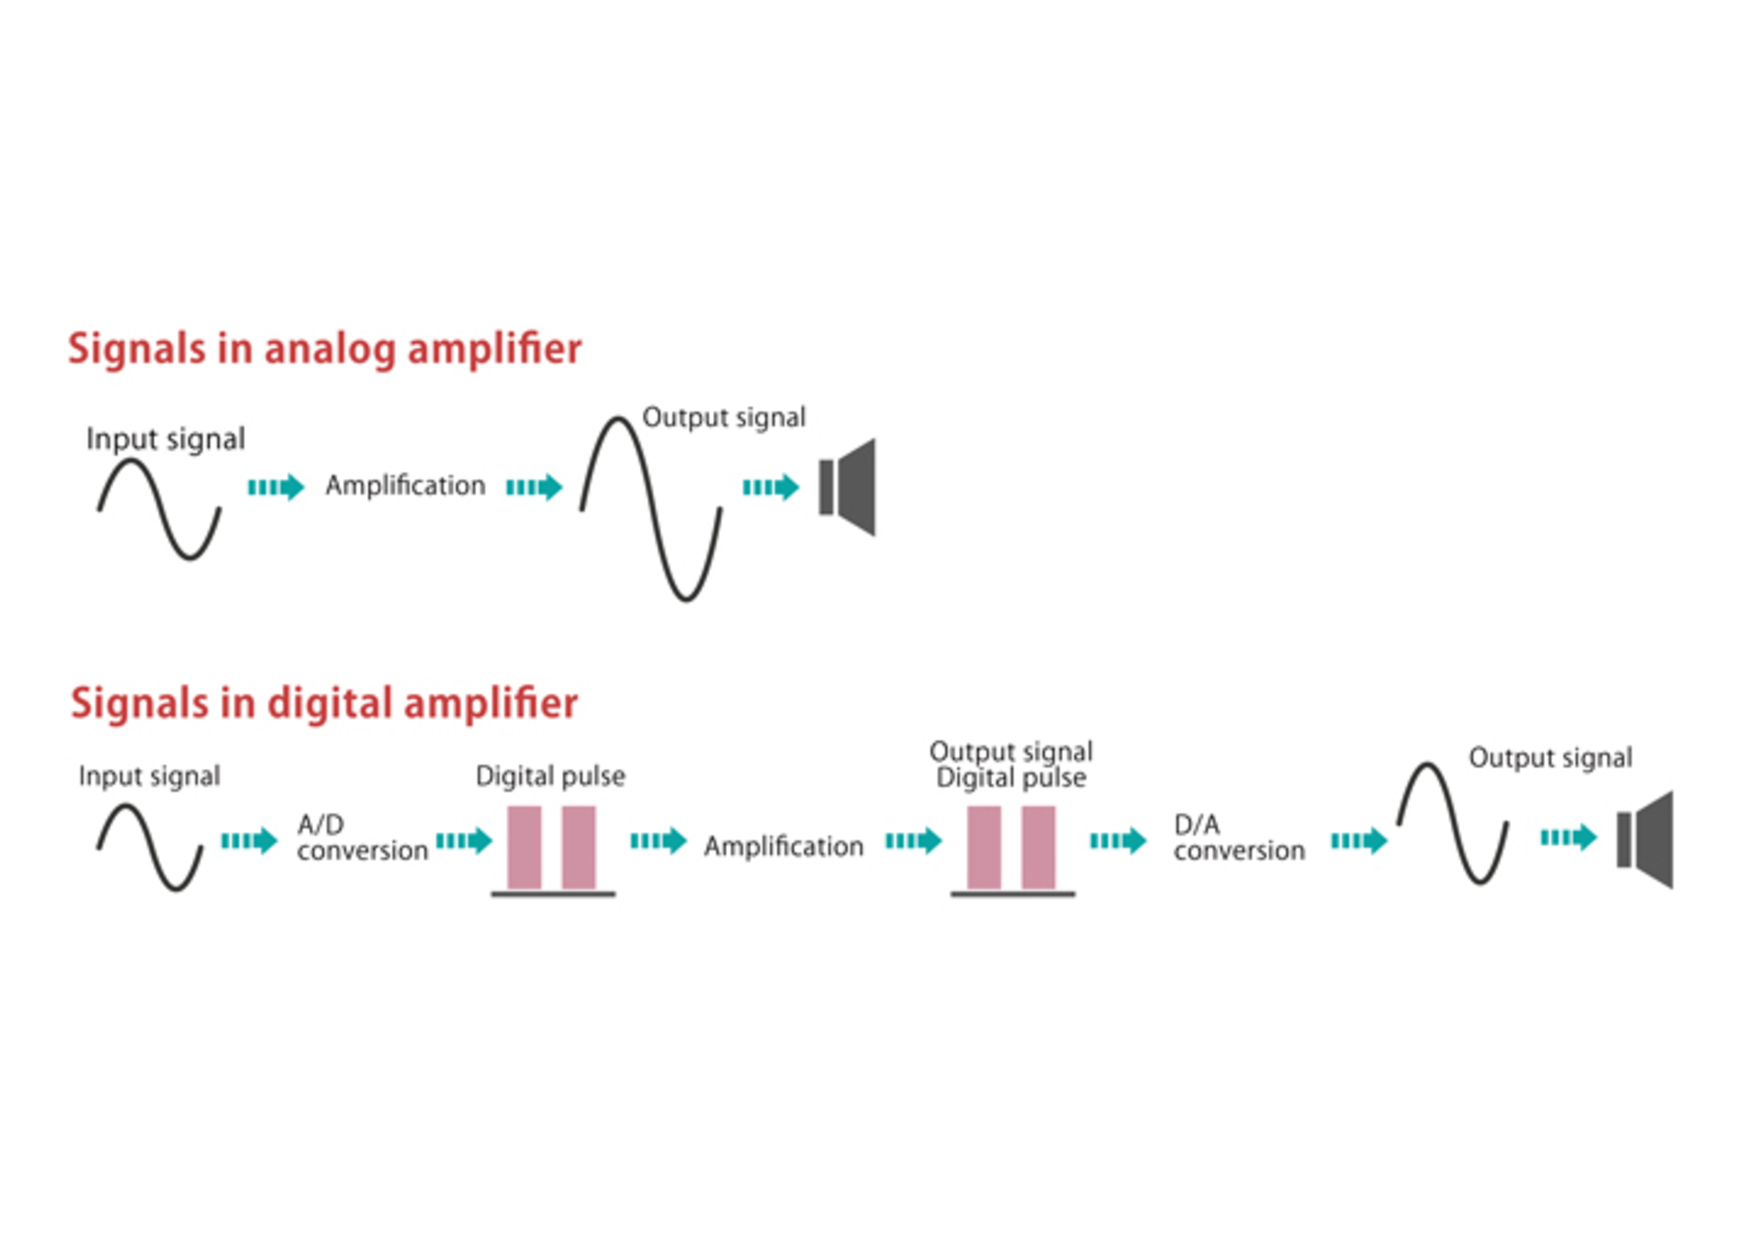
\includegraphics[scale=0.4]{Figures/Signal19.pdf}
%\end{figure}
%}

\frame{
\frametitle{Communication channel}
\begin{figure}
\centering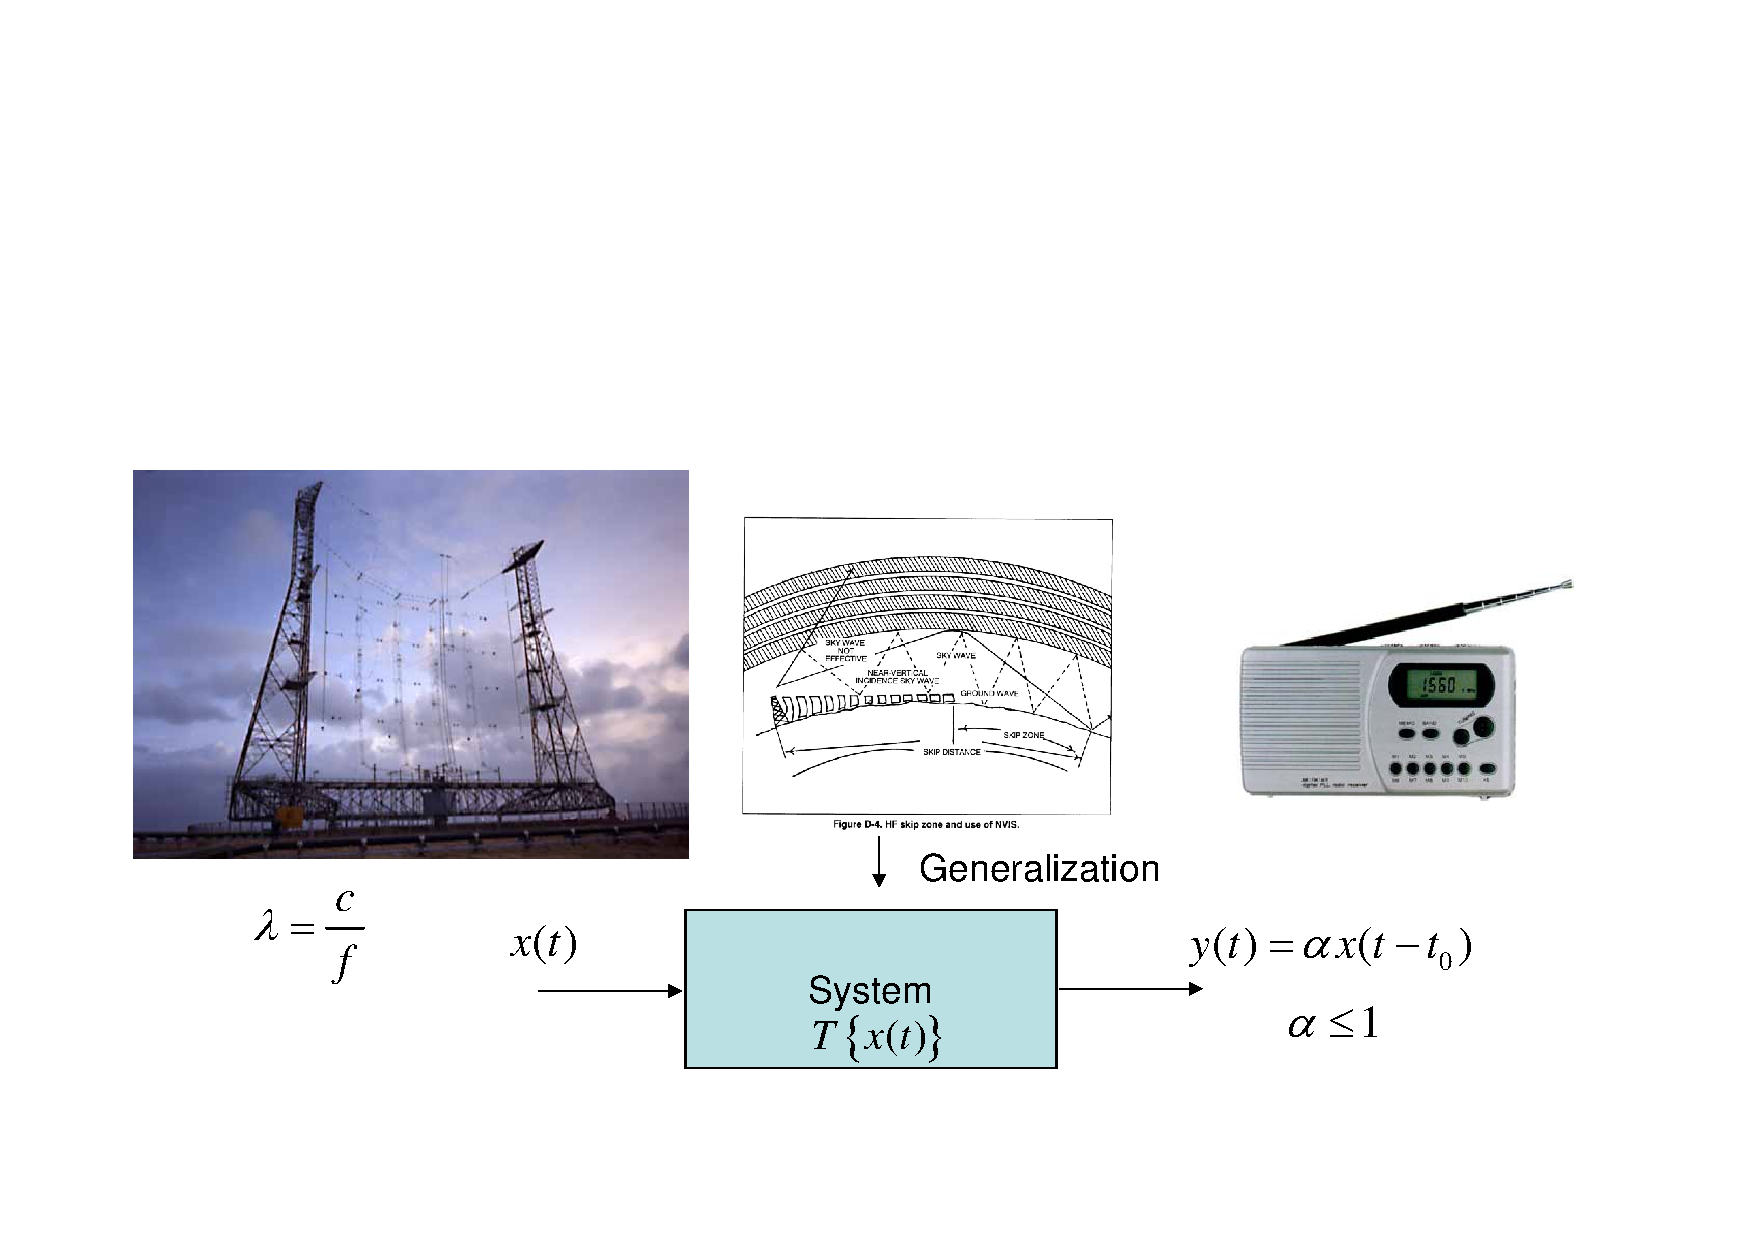
\includegraphics[scale=0.5]{Figures/Signal22.pdf}
\end{figure}
}

\frame{
\frametitle{Seismic analysis and earthquake prevention}
\begin{figure}
\centering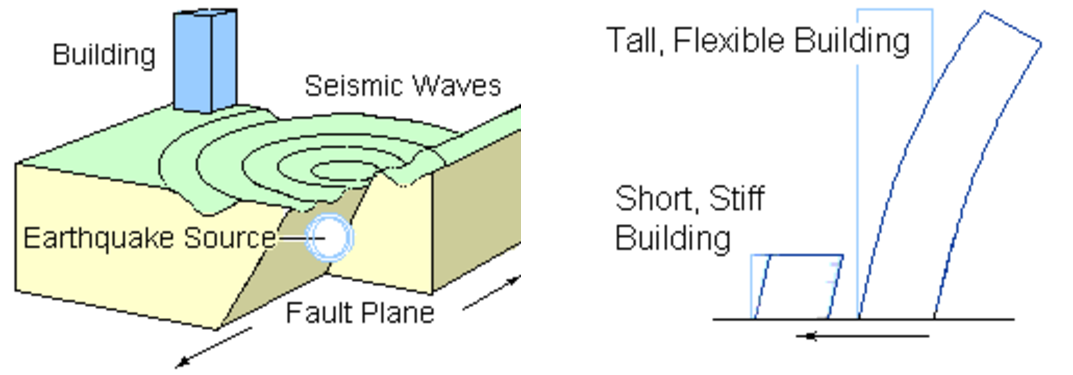
\includegraphics[scale=0.5]{Figures/Signal24.pdf}
\end{figure}
\begin{itemize}
\item The building can be seen as a system.
\item Input signal: seismic (sinusoidal) wave with amplitude $A$ and angular frequency $\omega$.
\item Output signal: Building curvature and displacement.
\end{itemize}
}

\frame{
\frametitle{Electric Circuits}
\begin{figure}
\centering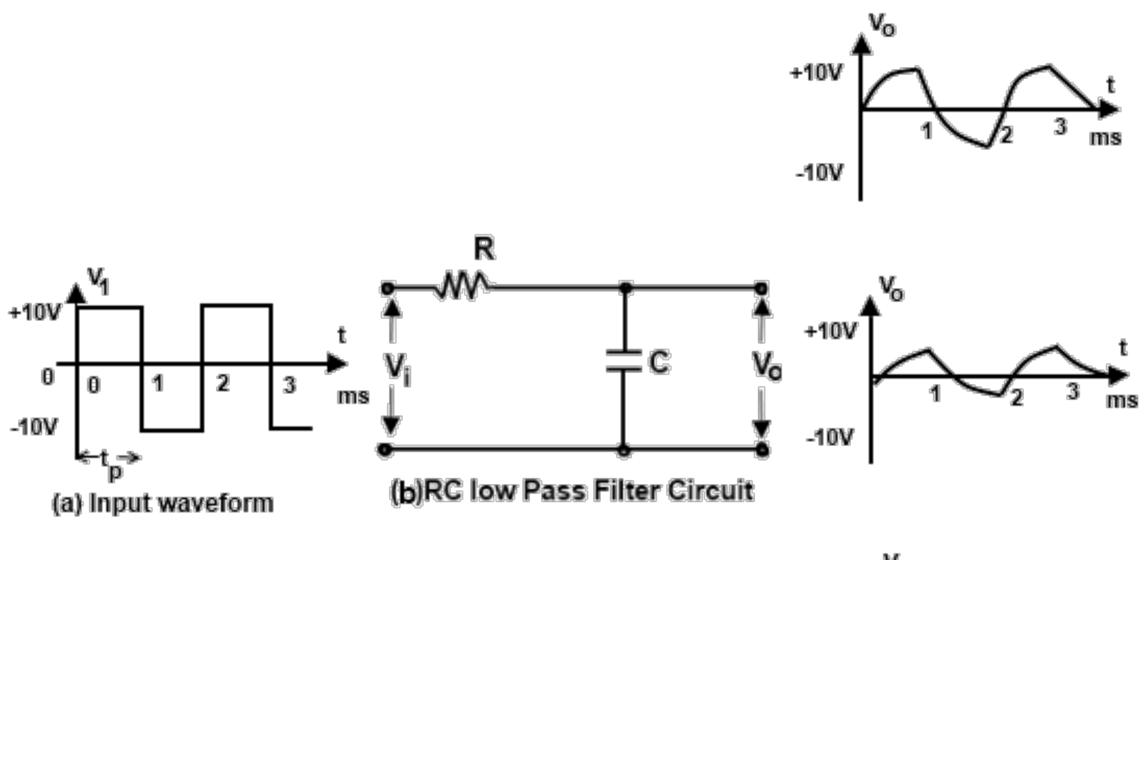
\includegraphics[scale=0.4]{Figures/Signal29.pdf}
\end{figure}
\begin{itemize}
\item Voltages and currents as a function of time in an electrical circuit are examples of signals. 
\item A circuit is itself an example of a system, which responds to applied input voltage/current signals.
\end{itemize}

}


\frame{
\frametitle{Motivation: Image Filtering}

\begin{figure}
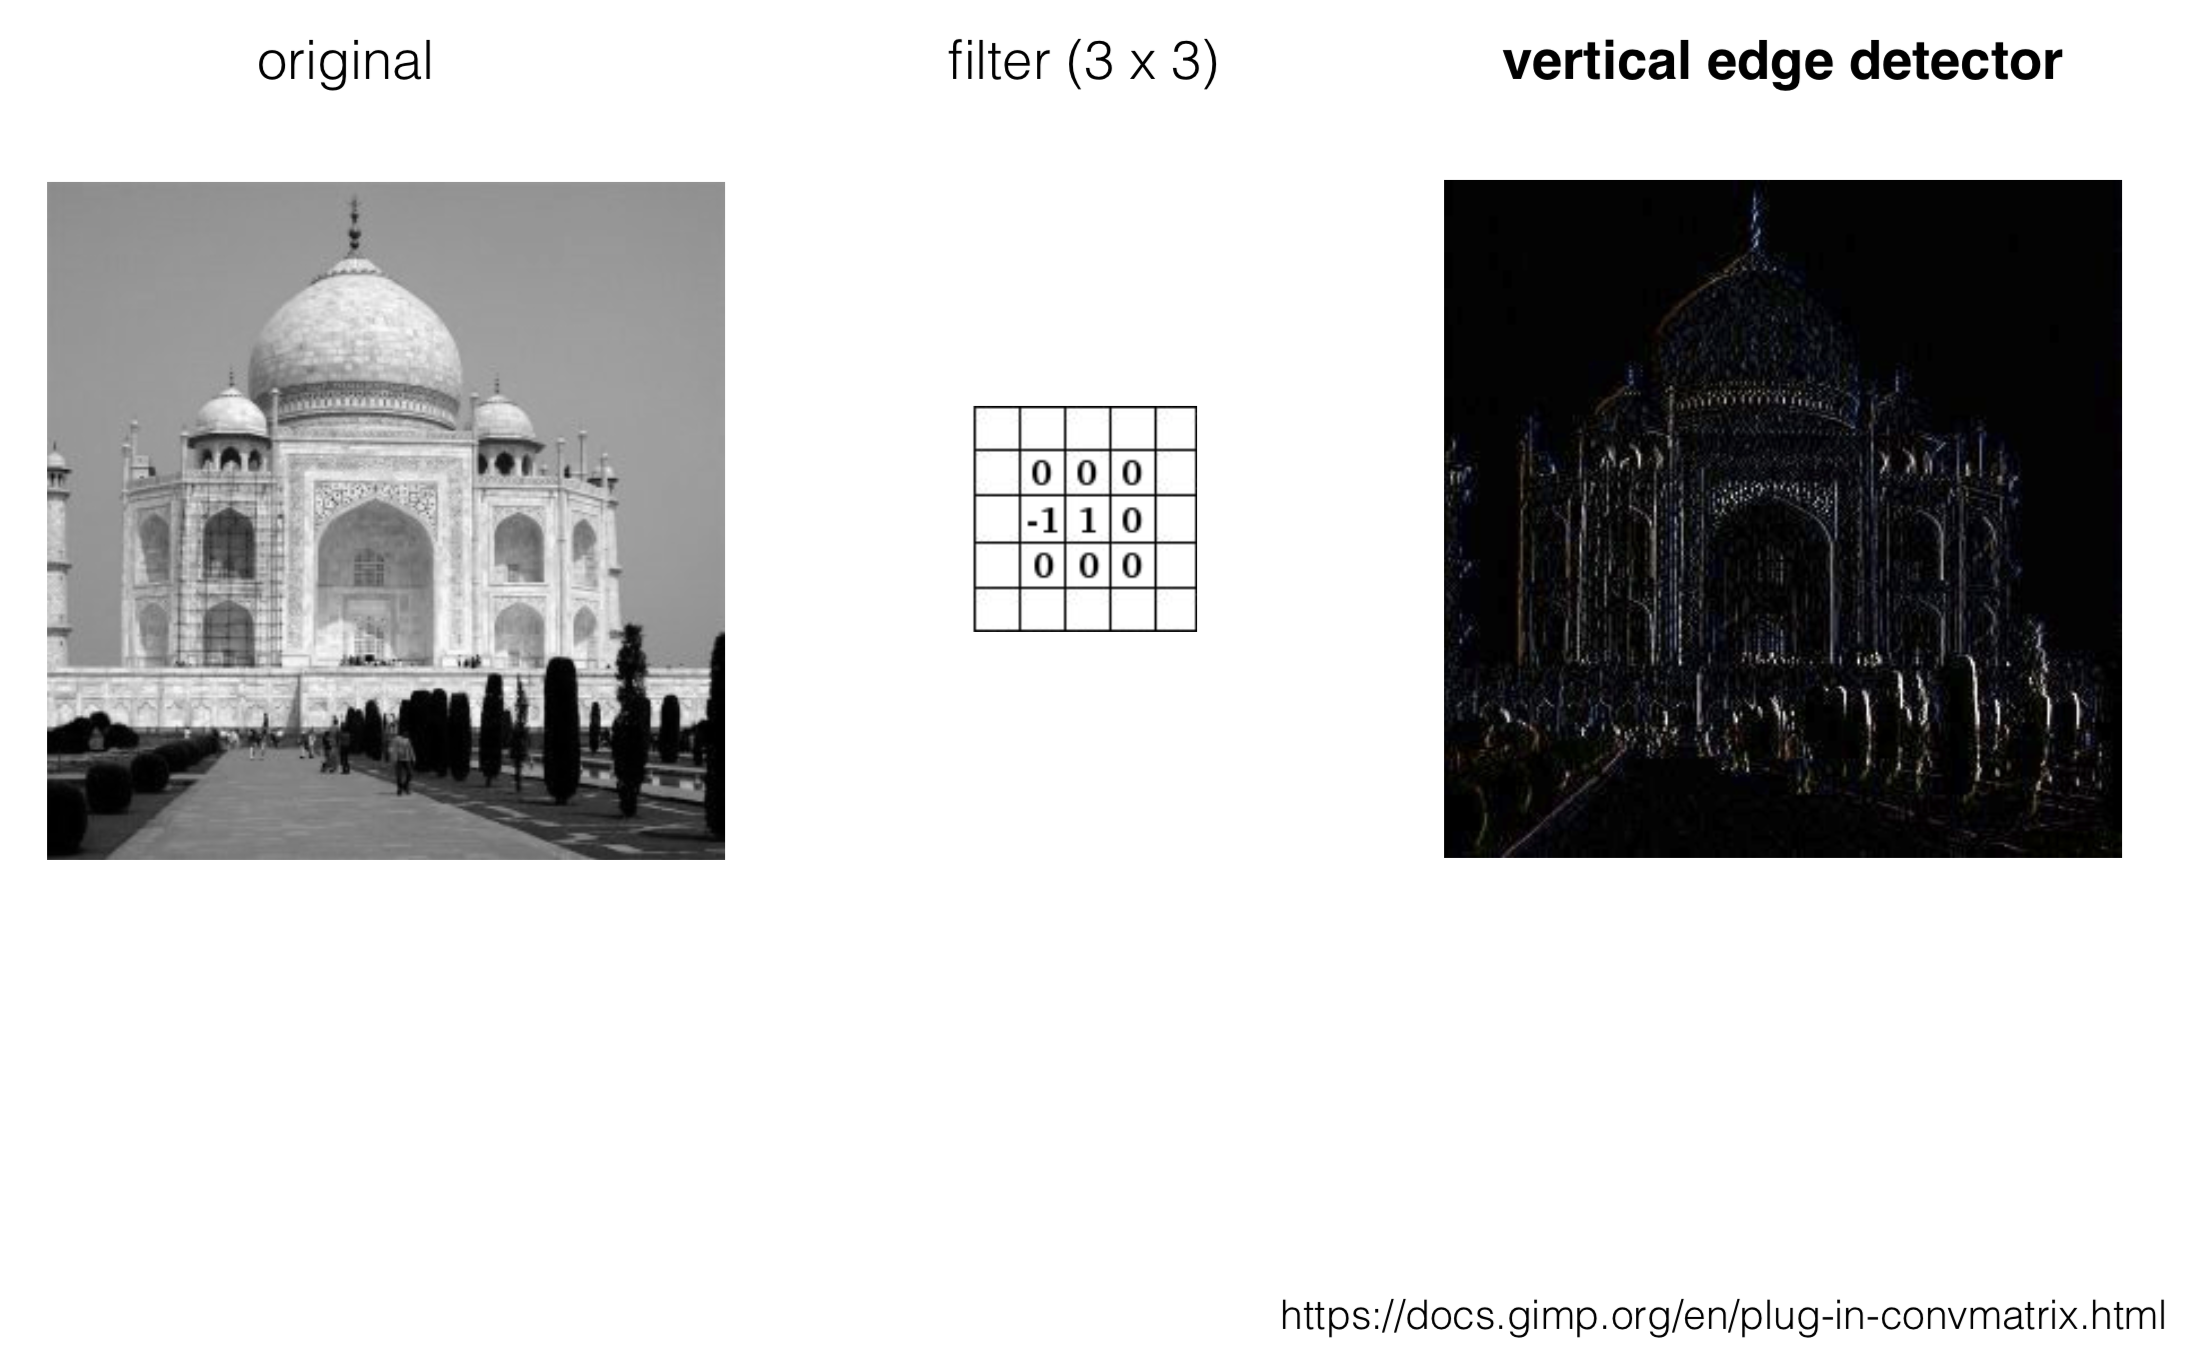
\includegraphics[scale=0.3]{Filtro_1.png}
\end{figure}

}

\frame{
\frametitle{Image Filtering}

\begin{figure}
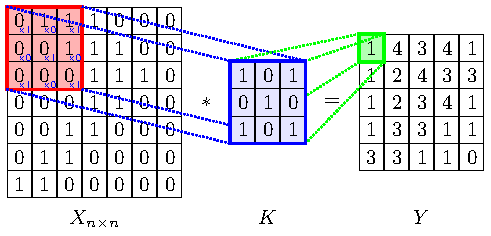
\includegraphics[scale=1.0]{2D_1.pdf}
\end{figure}

\begin{align*}
Y[1,1]&=X[1,1]*K[1,1]+X[1,2]*K[1,2]+X[1,3]*K[1,3]\\
&+X[2,1]*K[2,1]+X[2,2]*K[2,2]+X[2,3]*K[2,3]\\
&+X[3,1]*K[3,1]+X[3,2]*K[3,2]+X[3,3]*K[3,3]
\end{align*}
}

\frame{
\frametitle{Image Filtering}

\begin{figure}
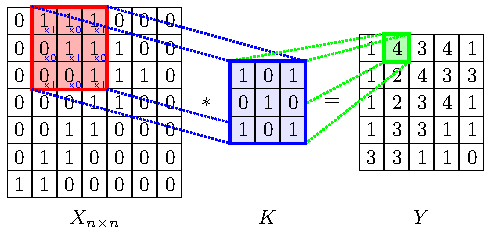
\includegraphics[scale=1.0]{2D_2.pdf}
\end{figure}

\begin{align*}
Y[1,2]&=X[1,2]*K[1,1]+X[1,3]*K[1,2]+X[1,4]*K[1,3]\\
&+X[2,2]*K[2,1]+X[2,3]*K[2,2]+X[2,4]*K[2,3]\\
&+X[3,2]*K[3,1]+X[3,3]*K[3,2]+X[3,4]*K[3,3]
\end{align*}
}




\frame{
\frametitle{Image Filtering}

\begin{figure}
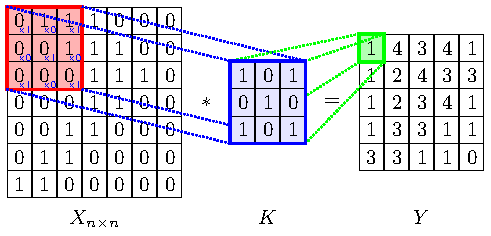
\includegraphics[scale=1.0]{2D_1.pdf}
\end{figure}

\begin{align*}
Y[i,j]&=\sum_{k_1=1}^{n}\sum_{k_2=1}^{n} X[k_1,k_2]K[i-k_1,j-k_2], ~~~ K[u,q]=0 \text{ para } u>3, q>3
\end{align*}

{\bf Linear operator, the result does not depend on the position of the image}
}

\frame{
\frametitle{Image Filtering}

\begin{figure}
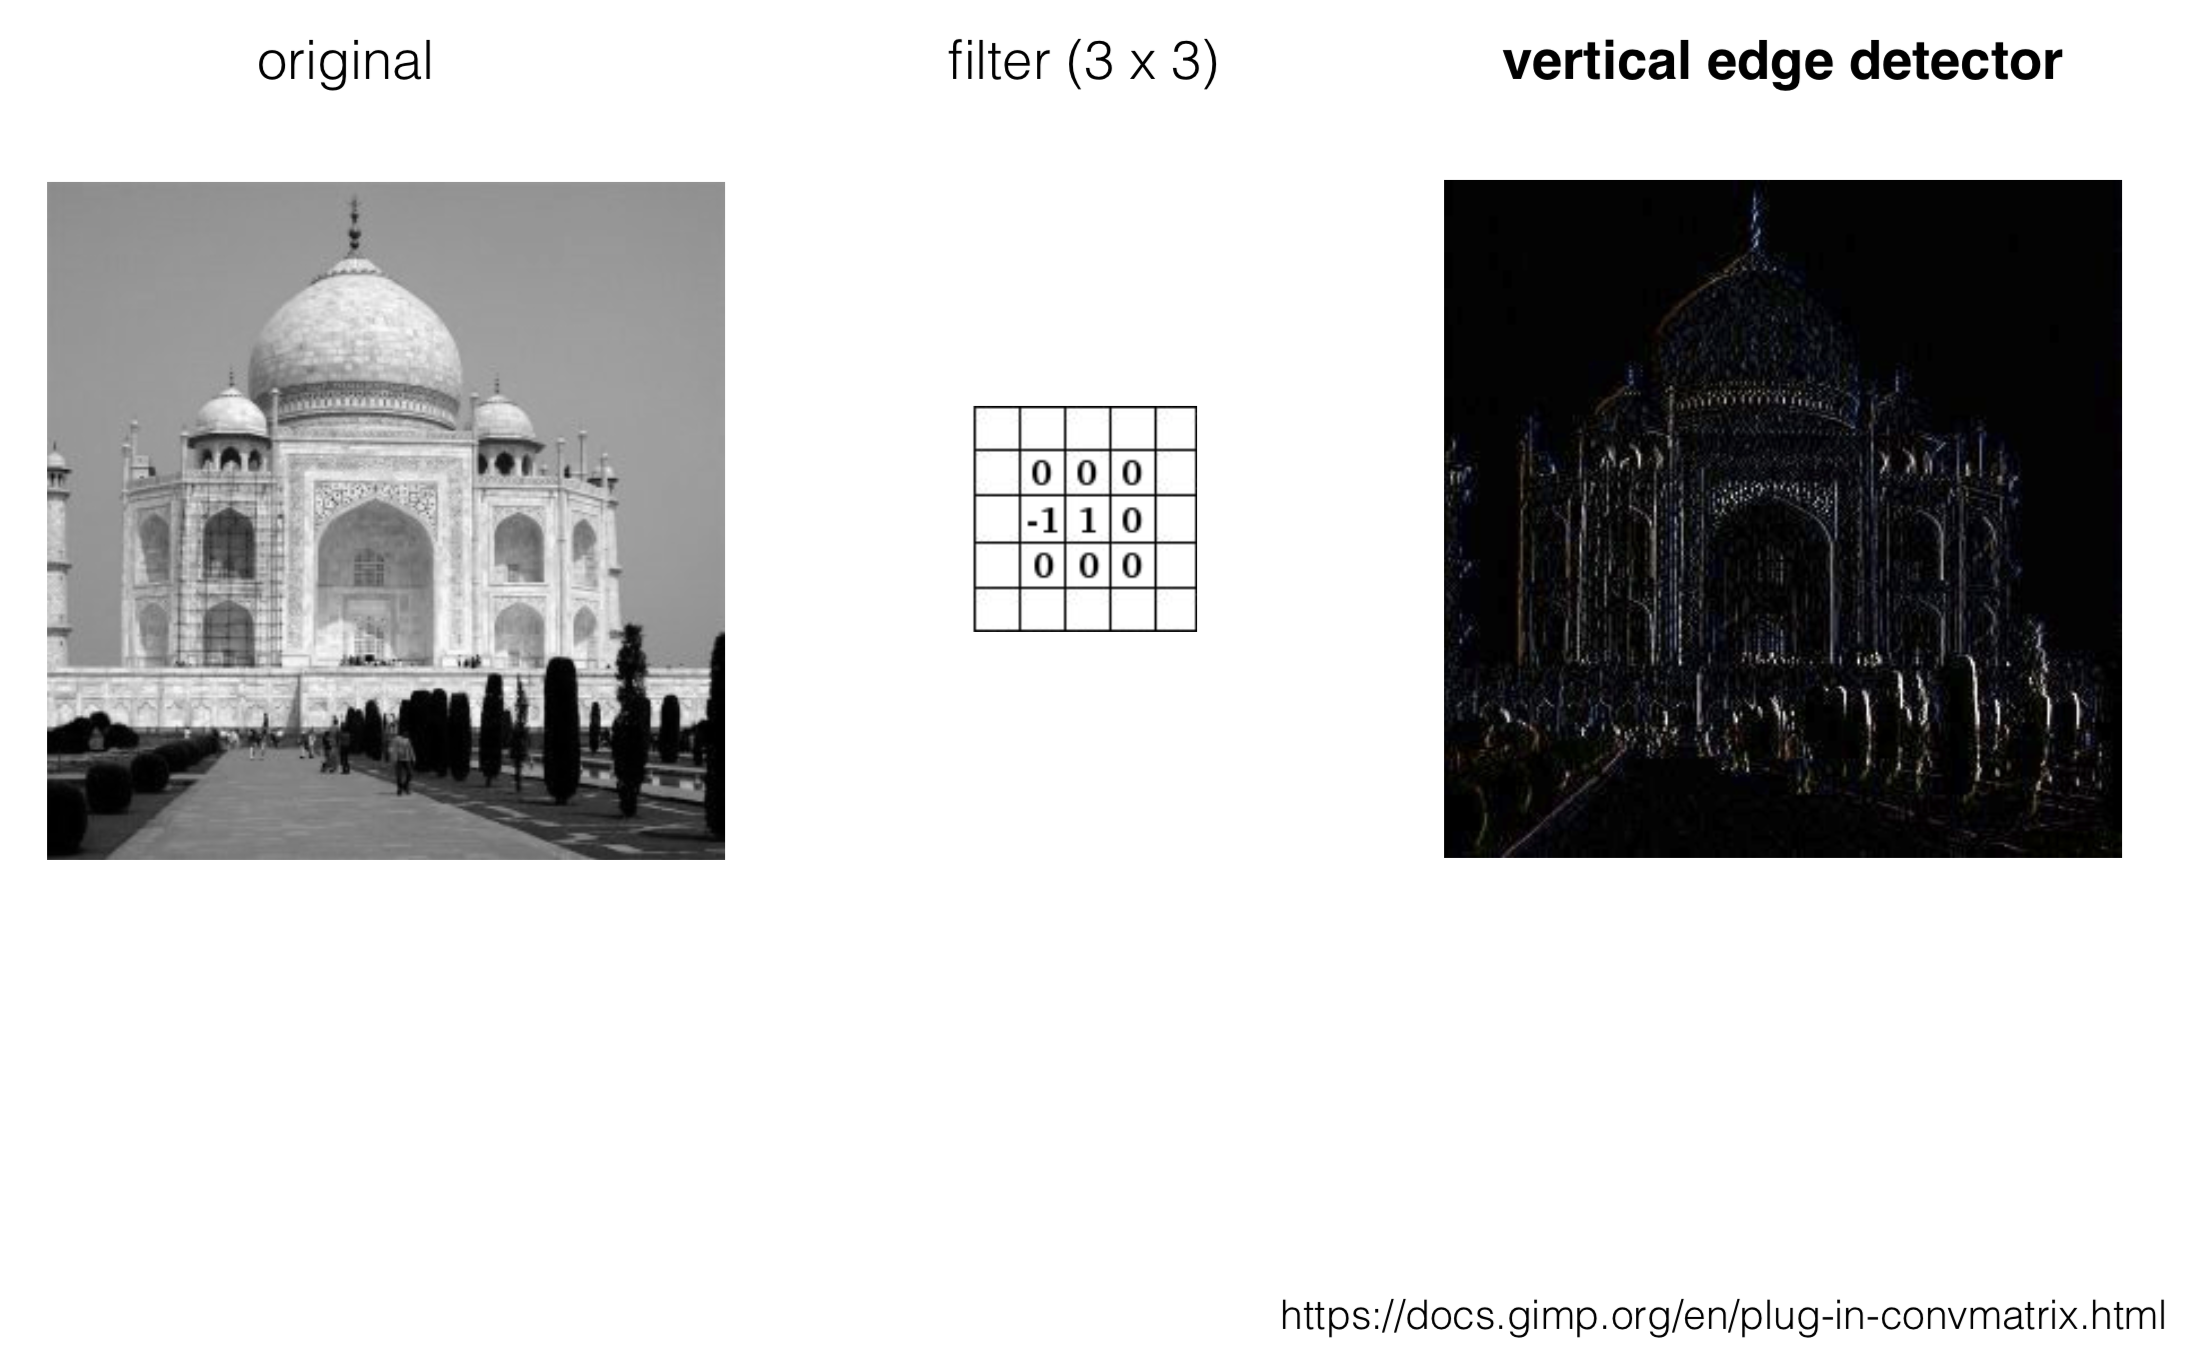
\includegraphics[scale=0.3]{Filtro_1.png}
\end{figure}

}

\frame{
\frametitle{Image Filtering}

\begin{figure}
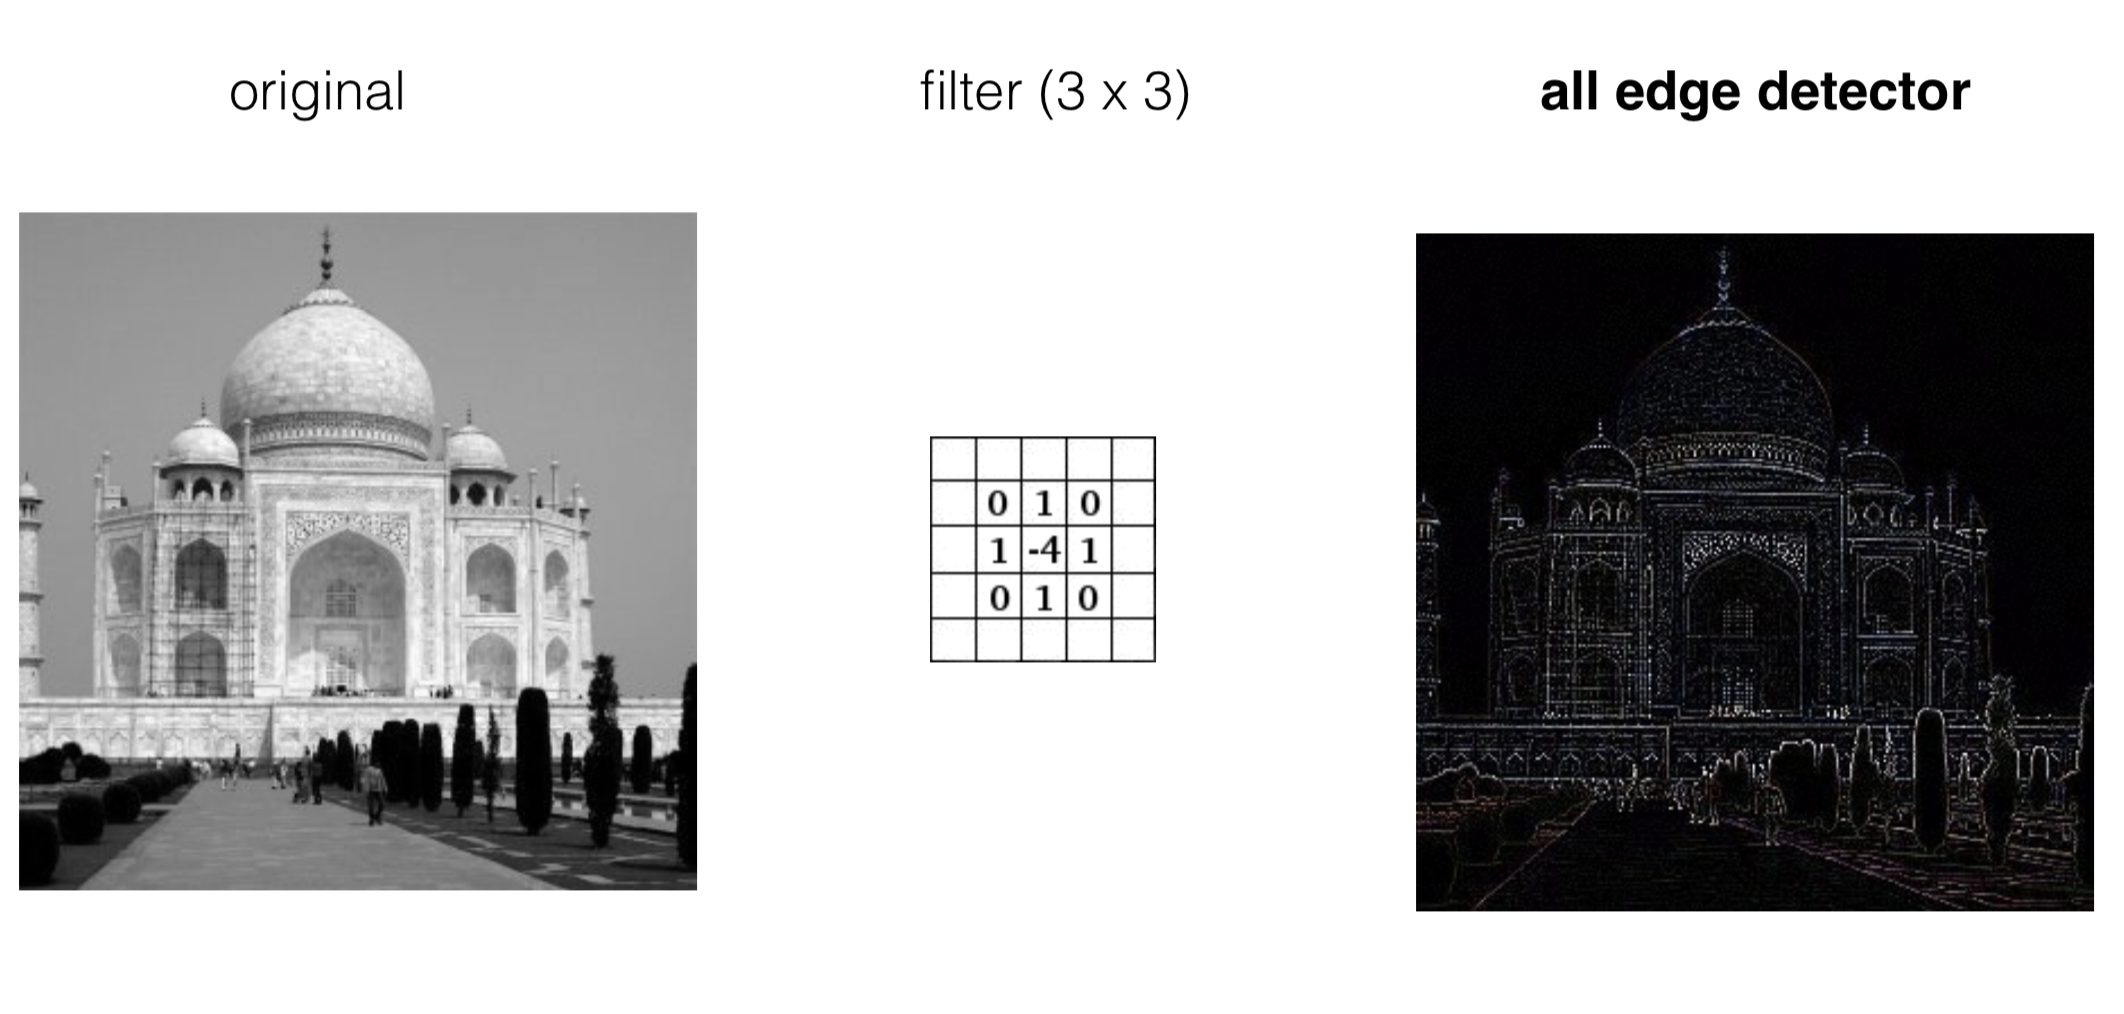
\includegraphics[scale=0.3]{Filtro_2.png}
\end{figure}

}

\frame{
\frametitle{Image Filtering}

\begin{figure}
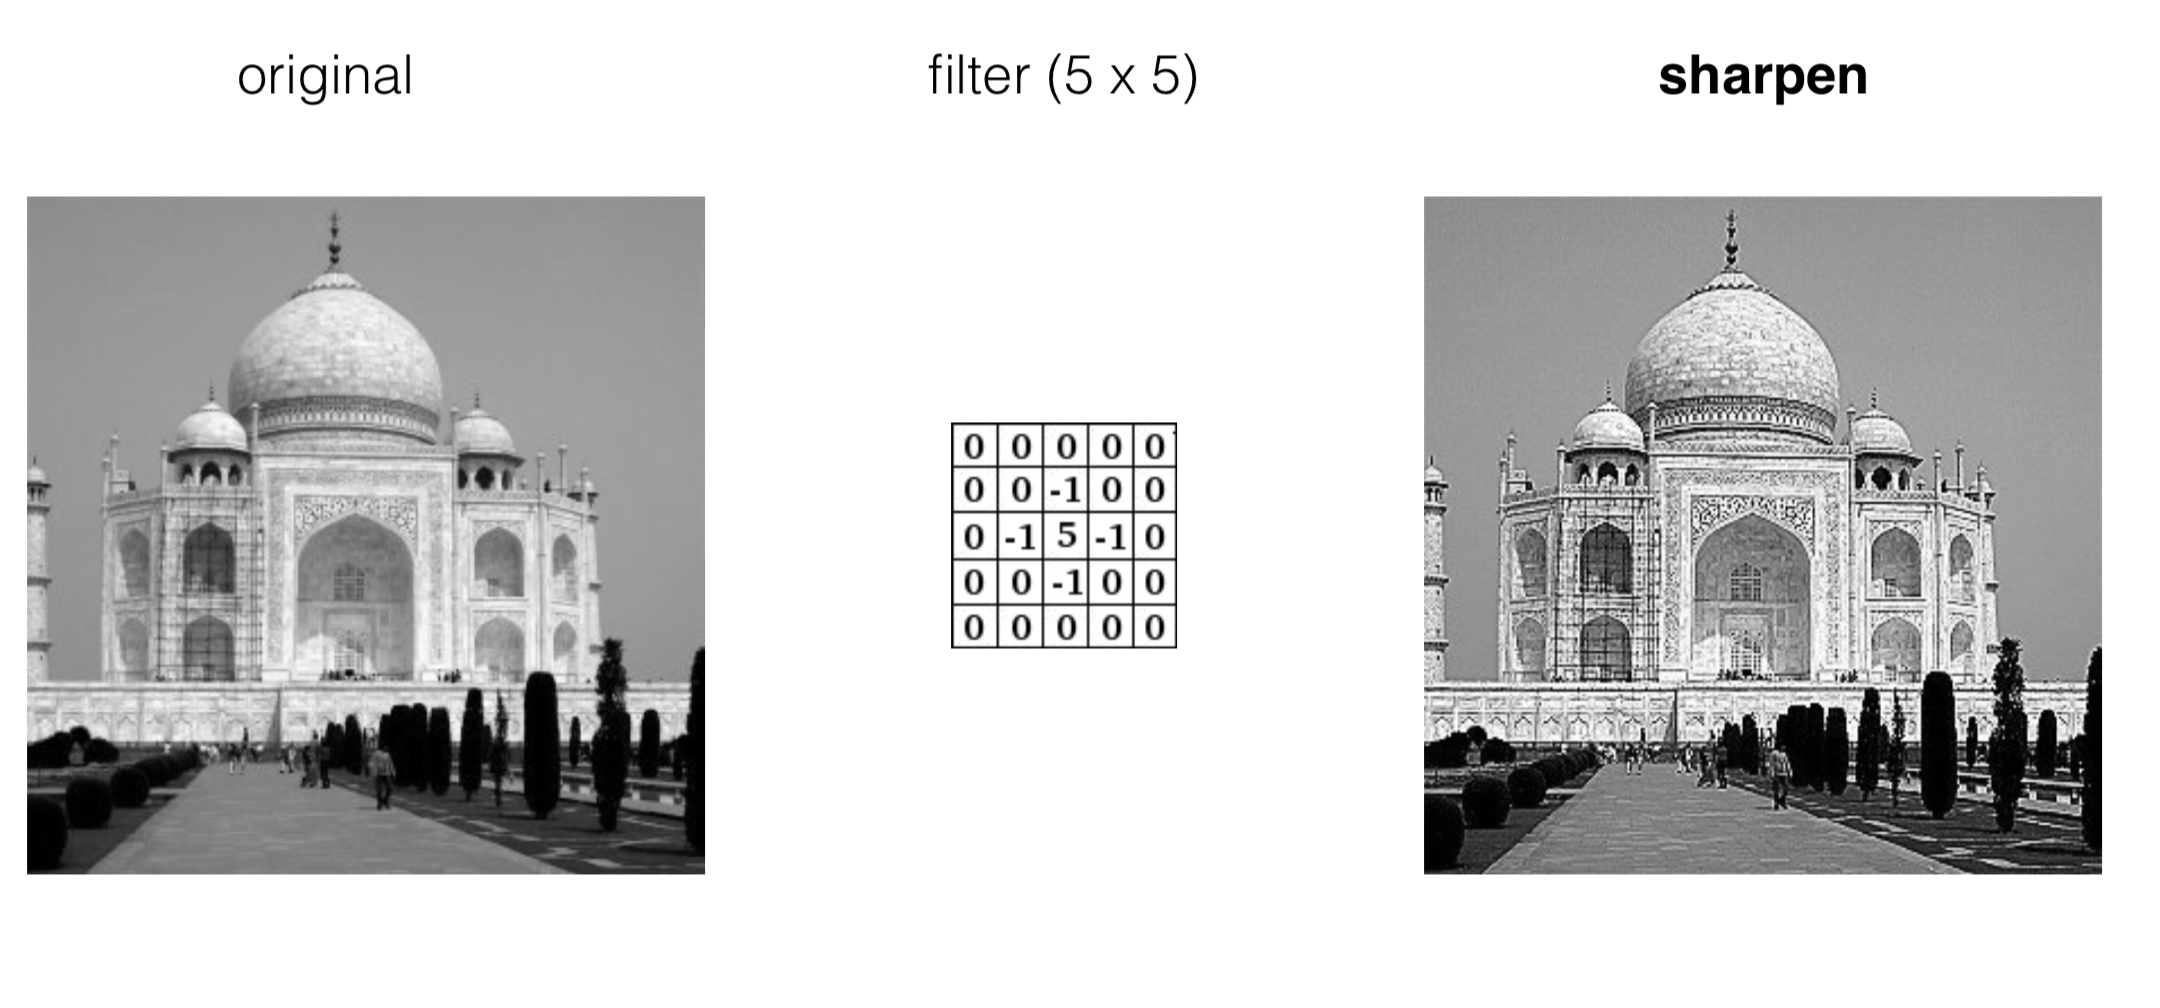
\includegraphics[scale=0.3]{Filtro_3.png}
\end{figure}

}

\section{Continuous-time and discrete-time systems}

\frame{

\begin{center}
\begin{tabular}{c}
\begin{pspicture}[](6,2)
   \pssignal(0,1){x}{$x(t)$}
   \psblock(3,1){a}{Continuous-time System}
   %\psblock(4,1){b}{$h[n], H(z)$}
   \pssignal(6,1){y}{$y(t)$}
   %-----------------
   \psset{arrows=->}
   \ncline{x}{a}  \ncline{a}{y}  %\ncline{b}{y}
\end{pspicture}
\\\\\\
\begin{pspicture}[](6,2)
   \pssignal(0,1){x}{$x[n]$}
   \psblock(3,1){a}{Discrete-time System}
   %\psblock(4,1){b}{$h[n], H(z)$}
   \pssignal(6,1){y}{$y[n]$}
   %-----------------
   \psset{arrows=->}
   \ncline{x}{a}  \ncline{a}{y}  %\ncline{b}{y}
\end{pspicture}
\end{tabular}
\end{center}

Symbolically, we represent a system as:
\begin{align}\nn
x(t)\rightarrow y(t)\\\nn
x[n]\rightarrow y[n]
\end{align}

}

\frame{
\frametitle{Interconnection of systems}

Complex system composed of the interconnection of simpler systems:


\begin{center}
\begin{tabular}{c}
\textbf{Cascade interconnection}\\\\
\begin{pspicture}[](8,2)
   \pssignal(0,1){x}{Input}
   \psblock(2,1){a}{System 1}
   \psblock(5,1){b}{System 2}
   \pssignal(8,1){y}{Output}
   %-----------------
   \psset{arrows=->}
   \ncline{x}{a}  \ncline{a}{b}  \ncline{b}{y}
\end{pspicture}
\\\\
\textbf{Parallel interconnection}\\\\
\begin{pspicture}[](6.5,2)
  %
   \pssignal(0,1){x}{Input}
   \pnode(1,1){b}
   \pnode(1,2){c}
   \pnode(1,0){d}
   \psblock(3,2){e}{System 1}
   \psblock(3,0){f}{System 2}
   \pnode(5,2){g}
   \pnode(5,0){h}
   \pscircleop(5,1){oplus}
   \pssignal(6.25,1){i}{Output}
   \ncline{x}{b}  \ncline{b}{c}  \ncline{b}{d}
    \ncline{e}{g} \ncline{f}{h}
    \psset{style=RoundCorners ,style=Arrow}	
     \ncline{c}{e} \ncline{d}{f}
   \ncline{g}{oplus}  \ncline{h}{oplus} \ncline{oplus}{i}
\end{pspicture}
\end{tabular}
\end{center}

}

\frame{
\frametitle{Interconnection of systems}

\begin{center}
\begin{tabular}{c}
\textbf{Series/Parallel interconnection}\\\\
\begin{pspicture}[](8,2)
	
   \pssignal(0,1){x}{Input}
   \pnode(1,1){b}
   \pnode(1,2){c}
   \pnode(1,0){d}
   \psblock(2.5,2){e}{System 1}
   \psblock(5,2){j}{System 2}
   \psblock(4,0){f}{System 3}
   \pnode(6.5,2){g}
   \pnode(6.5,0){h}
   \pscircleop(6.5,1){oplus}
   \pssignal(8,1){i}{Output}
   
   %Conexiones
   \ncline{x}{b}  \ncline{b}{c}  \ncline{b}{d}
     \ncline{f}{h} \ncline{j}{g}
   \psset{style=RoundCorners ,style=Arrow}
     \ncline{c}{e} \ncline{d}{f}
   \ncline{g}{oplus}  \ncline{h}{oplus} \ncline{oplus}{i}
   \ncline{e}{j}
\end{pspicture}
\end{tabular}
\end{center}

\begin{block}{}
In general, the order is NOT interchangeable.
\end{block}

}

\frame{
\begin{align}\nn
y[n]=(2x[n]-x^2[n])^2
\end{align}
\vspace{1cm}

\begin{center}
\begin{pspicture}[](7.5,2)
	
   \pssignal(0,1){x}{$x[n]$}
   \pnode(1,1){b}
   \pnode(1,2){c}
   \pnode(1,0){d}
   \psblock(3,2){e}{Multiply by 2}
   \psblock(3,0){f}{Square}
   \pnode(5,2){g}
   \pnode(5,0){h}
   \pscircleop(5,1){oplus}
   \psblock(6.25,1){j}{Square}
   \pssignal(8.25,1){i}{$y[n]$}
   \ncline{x}{b}  \ncline{b}{c}  \ncline{b}{d}
    \ncline{e}{g} \ncline{f}{h}
   \psset{style=RoundCorners ,style=Arrow}
     \ncline{c}{e} \ncline{d}{f}
      \ncline{oplus}{j} \ncline{j}{i}
   \ncstar{->}{ncline}[naput]{h -}{oplus} %\ncline{h}{oplus}
   \ncline{g}{oplus}
\end{pspicture}
\end{center}

}

\frame{
\frametitle{Problem 31}

Consider the following interconnection of systems:

\begin{center}
\begin{pspicture}[](8,2)
   \pssignal(0,1){x}{$x(t)$}
   \pnode(1,1){b}
   \pnode(1,2){c}
   \pnode(1,0){d}
   \psblock(2.5,2){e}{$T_1$}
   \psblock(5,2){j}{$T_2$}
   \psblock(4,0){f}{$T_3$}
   \pnode(6.5,2){g}
   \pnode(6.5,0){h}
   \pscircleop(6.5,1){oplus}
   \pssignal(8,1){i}{$y(t)$}
   %Conexiones
   \ncline{x}{b}  \ncline{b}{c}  \ncline{b}{d}
     \ncline{f}{h} \ncline{j}{g}
   \psset{style=RoundCorners ,style=Arrow}
     \ncline{c}{e} \ncline{d}{f}
   \ncline{g}{oplus}  \ncline{h}{oplus} \ncline{oplus}{i}
   \ncline{e}{j}
\end{pspicture}
\end{center}
where $T_1: y(t)=2x(t-2)$, $T_2: y(t)=dx(t-2)/dt$ and $T_3: y(t)=x(-t+1)$.
\begin{enumerate}[a)]
\item Determine the system input-output relationship.
\item Compute the system response when $x(t)=u(t)$.
\end{enumerate}


}

\frame{
Sol:

\begin{center}
\begin{pspicture}[](8,2)

   \pssignal(0,1){x}{$x(t)$}
   \pnode(1,1){b}
   \pnode(1,2){c}
   \pnode(1,0){d}
   \psblock(2.5,2){e}{$T_1$}
   \psblock(5,2){j}{$T_2$}
   \psblock(4,0){f}{$T_3$}
   \pnode(6.5,2){g}
   \pnode(6.5,0){h}
   \pscircleop(6.5,1){oplus}
   \pssignal(8,1){i}{$y(t)$}
      \pssignal(3.75,2.3){}{$e(t)$}
   \pssignal(6,2.3){}{$w(t)$}
   \pssignal(6,-0.3){}{$r(t)$}
   %Conexiones
   \ncline{x}{b}  \ncline{b}{c}  \ncline{b}{d}
     \ncline{f}{h} \ncline{j}{g}
   \psset{style=RoundCorners ,style=Arrow}
     \ncline{c}{e} \ncline{d}{f}
   \ncline{g}{oplus}  \ncline{h}{oplus} \ncline{oplus}{i}
   \ncline{e}{j}
\end{pspicture}
\end{center}

\begin{align*}
&e(t)=2x(t-2)\Rightarrow ~ w(t)=\frac{de(t-2)}{d t}=2\frac{dx(t-4)}{d t}\\
&r(t)=x(-t+1)
%&\Rightarrow y(t)=2\frac{dx(t-4)}{d t}+x(-t+1)
\end{align*}

\begin{exampleblock}{For $x(t)=u(t)$}
\begin{align*}
y(t)=2\frac{dx(t-4)}{d t}+x(-t+1)= 2 \delta(t-4)+u(-t+1)
\end{align*}
\end{exampleblock}


}


\section{Properties of systems}

\frame{
\frametitle{Systems with and without memory}

\begin{exampleblock}{}
A system $x(t)\rightarrow y(t)$ is said to be memoryless if the output $y(t_0)$ a one time instant $t_0$ only depends on the input at the same time instant, i.e.,  $x(t_0)$.
\end{exampleblock}

\textbf{Examples:}

\begin{itemize}
\item $y[n]=(2x[n]-x[n]^2)^2$ is memoryless.
\item $y(t)=x(t-1)$ is a system with memory.
\item $y(t)=x(t-3)x(t+2)$ is a system with memory.
\end{itemize}

}

\frame{
\frametitle{$y(t)=\frac{\partial x(t)}{\partial t}$ is a system \textcolor{red}{\textbf{with memory}}.}

\begin{align*}
y(t)=\frac{\partial x(t)}{\partial t}\doteq \lim_{\Delta\rightarrow 0}\frac{x(t+\Delta)-x(t)}{\Delta}
\end{align*}

\begin{itemize}
\item We need $x(t+\Delta)$!
\item The system has memory!
\end{itemize}

}

\frame{
\frametitle{Invertibility and inverse systems}

\begin{block}{}
\begin{itemize}
\item A system is said to be invertible if distinct inputs lead to distinct outputs.
\item By observing its output, we can determine its input. 
\end{itemize}
\end{block}

\begin{tabular}{c}
\\\\
\begin{pspicture}[](9,2)
   \pssignal(0,1){x}{$x(t)$}
   \psblock(2,1){a}{$y(t)=2x(t)$}
   \psblock(5.5,1){b}{$z(t)=\frac{1}{2}y(t)$}
   \pssignal(8.25,1){y}{$x(t)$}
   %-----------------
   \psset{arrows=->}
   \ncline{x}{a}   \ncline{b}{y}
   \ncstar{->}{ncline}[naput]{a $y(t)$}{b} %\ncline{h}{oplus}
\end{pspicture}
\\\\
\begin{pspicture}[](13,2)
   \pssignal(0,1){x}{$x[n]$}
   \psblock(3,1){a}{$y[n]=\sum_{k=-\infty}^{n}x[k]$}
   \psblock(8,1){b}{$z[n]=y[n]-y[n-1]$}
   \pssignal(11,1){y}{$x[n]$}
   %-----------------
   \psset{arrows=->}
   \ncline{x}{a}   \ncline{b}{y}
    \ncstar{->}{ncline}[naput]{a $y[n]$}{b} %\ncline{h}{oplus}
\end{pspicture}
\end{tabular}
}

\frame{

Are invertible the following systems?

\begin{itemize}
\item $y[n]=x[2n]$
\item $y(t)=x(2t)$
\item $y(t)=x^{2}(t)$
\end{itemize}

}

\frame{
\frametitle{Problem 33}

Consider the following discrete-time system 
\begin{align*}
y[n]=x[n]x[n-2]
\end{align*}
\begin{enumerate}[a)]
\item Is the system memoryless?
\item Determine the system response when the input is $x[n]=A\delta[n]$, where $A\in\mathbb{C}$.
\item Is the system invertible?
\end{enumerate}

}

\frame{
\frametitle{Causality}

\begin{exampleblock}{}
\begin{itemize}
\item A system is causal if the output at any time depends only on values of the input at the present time and in the past. 
%\item A causal system is also referred to as nonanticipative.
\item $y(t)=f(x(t))$ is causal if $y(t_0)$ only depends on $x(t)$ for $t\leq t_0$.
\item $y[n]=f(x[n])$ is causal if $y[n_0]$ only depends on $x[n]$ for $n\leq n_0$.
\item Memoryless systems are always causal.
\end{itemize}
\end{exampleblock}



}

\frame{
Are the following systems causal?
\begin{itemize}
\item $y[n]=x[n]-x[n+1]$ 
\item $y(t)=x(t+1)$ 
\item $y[n]=\text{Even}(x[n-1])$?
\item $y(t)=x(\sin(t))$
\end{itemize}


}

\frame{
\frametitle{Stability}

\begin{exampleblock}{Bounded signal}
Consider an input signal $x(t)$ that verifies
\begin{align*}
|x(t)|\leq B~~\forall t
\end{align*}
for some real constant $B$. We say $x(t)$ is a bounded signal.
\end{exampleblock}

\begin{block}{Bounded Input, Bounded Output (BIBO) stability}
A given system $x(t)\rightarrow y(t)$ is \textbf{BIBO stable} if there exists a real constant $C$ for which 
\begin{align*}
|y(t)|\leq C ~~\forall t
\end{align*}
for any input signal $x(t)$ that is bounded.
\end{block}
Same definition holds for discrete-time systems.

}

\frame{

Determine whether the following systems are stable:
\begin{align*}
y(t)&=x(t/3)\\\\
y[n]&=nx[n]\\\\
y(t)&=\int_{t-2}^{t-1}x^3(\tau)d\tau\\\\\
y[n]&=\sum_{k=-\infty}^{n}(1/2)^{n-k} x[k]
\end{align*}


}

\frame{
\frametitle{Time Invariance}

\begin{block}{}
A system is time-invariant if a time shift in the input signal causes a time shift in the output signal.
\end{block}
\vspace{0.5cm}

\begin{itemize}
\item If $y[n]=f(x[n])$, the system is invariant if $f(x[n-n_0])=y[n-n_0]$. 
\item If $y(t)=f(x(t))$, the system is invariant if $f(x(t-t_0))=y(t-t_0)$. 
\end{itemize}
}

\frame{
\frametitle{$y(t)=\sin(x(t))$}

Let $x_1(t)$ be the input:
\begin{align}\nn
y_1(t)=\sin(x_1(t)).
\end{align}
Define $x_2(t)=x_1(t-t_0)$:
\begin{align}\nn
y_2(t)=\sin(x_2(t))=\sin(x_1(t-t_0))=y_1(t-t_0).
\end{align}
The system is time-invariant.

}

\frame{
\frametitle{$y[n]=nx[n]$}
Let $x_1[n]$ be the input:
\begin{align}\nn
y_1[n]=nx_1[n].
\end{align}
Define $x_2[n]=x_1[n-n_0]$:
\begin{align}\nn
&y_2[n]=nx_2[n]=nx_1[n-n_0]\\\nn
 &y_1[n-n_0]=(n-n_0)x_1[n-n_0].
\end{align}
Therefore
\begin{align*}
y_1[n-n_0]�~~\mathbf{\neq}~~ y_2[n]
\end{align*}
The system is NOT time-invariant.


}

\frame{
\frametitle{Linearity}
Linear systems posse the important property of \textbf{superposition}.

\begin{exampleblock}{}
 For any system, consider two arbitrary inputs and their respective outputs:
\begin{align}\nn
x_1(t)\rightarrow y_1(t)\\\nn
x_2(t)\rightarrow y_2(t),
\end{align}
the system is linear if 
\begin{align}\nn
ax_1(t)+bx_2(t)\rightarrow ay_1(t)+by_2(t)
\end{align}
for any two complex constants $a,b\in\mathbb{C}$.
\end{exampleblock}

\begin{block}{Linear discrete-time signals}
\begin{align}\nn
ax_1[n]+bx_2[n]\rightarrow ay_1[n]+by_2[n]
\end{align}
\end{block}

}

\frame{
The systems 
\begin{align}\nn
y[n]=(x[n])^{2},\\\nn
y[n]=\exp(x[n]),
\end{align}
are not linear. 
\vspace{0.5cm}

The system
\begin{align}\nn
y[n]=x[n]-x[n-3]+4x[n-8]
\end{align}
is linear.

}



%\frame{
%Videos about signals and systems with examples (University of Arizona State):
%
%\begin{exampleblock}{}
%\url{https://sites.google.com/a/asu.edu/signals-and-systems/\#TOC-System-Properties}
%\end{exampleblock}
%
%}


\end{document}
